% Project write-up adapted from the supplied CVPR 2026 main.tex template.
% Compile from this directory: pdflatex main; bibtex main; pdflatex main; pdflatex main
\documentclass[10pt,twocolumn,letterpaper]{article}

% The supplied template uses the CVPR style. This is a project report, not a
% CVPR submission, so the final style shows the author's name.
\usepackage[pagenumbers]{cvpr}
%% This file contains a number of tweaks that are typically applied to the main document.
%% They are not enabled by default, but can be enabled by uncommenting the relevant lines.

%%
%% Inline annotations; for predefined colors, refer to "dvipsnames" in the xcolor package:
%% https://tinyurl.com/overleaf-colors
%%
\newcommand{\red}[1]{{\color{red}#1}}
\newcommand{\todo}[1]{{\color{red}#1}}
\newcommand{\TODO}[1]{\textbf{\color{red}[TODO: #1]}}
%%
%% disable for camera ready / submission by uncommenting these lines
%%
% \renewcommand{\TODO}[1]{}
% \renewcommand{\todo}[1]{#1}

%%
%% work harder in optimizing text layout. Typically shrinks text by 1/6 of page, enable
%% it at the very end of the writing process, when you are just above the page limit
%%
% \usepackage{microtype}

%%
%% fine-tune paragraph spacing
%%
% \renewcommand{\paragraph}[1]{\vspace{.5em}\noindent\textbf{#1.}}

%%
%% globally adjusts space between figure and caption
%%
% \setlength{\abovecaptionskip}{.5em}


%%
%% Allows "the use of \paper to refer to the project name"
%% with automatic management of space at the end of the word
%%
% \usepackage{xspace}
% \newcommand{\paper}{ProjectName\xspace}

%%
%% Commonly used math definitions
%%
% \DeclareMathOperator*{\argmin}{arg\,min}
% \DeclareMathOperator*{\argmax}{arg\,max}

%%
%% Tigthen underline
%%
% \usepackage{soul}
% \setuldepth{foobar}

\usepackage{listings}
\usepackage[pagebackref,breaklinks,colorlinks,allcolors=blue]{hyperref}

\def\confName{Project Report}
\def\confYear{2026}
\title{Pimple Removal Tool: Acne Detection and Shared-Mask Image Inpainting}
\author{Yogdeep Singh Rajawat\\
\texttt{github.com/blackleg-sanji007}}

\lstset{
    basicstyle=\ttfamily\footnotesize,
    breaklines=true,
    breakatwhitespace=false,
    columns=fullflexible,
    frame=single,
    numbers=left,
    numberstyle=\tiny,
    numbersep=5pt,
    showstringspaces=false,
    tabsize=4
}

\begin{document}
\maketitle

\begin{abstract}
Acne removal from photographs requires two distinct decisions: which pixels
contain lesions and how to reconstruct plausible skin after those pixels are
removed. A restoration model applied to the whole face can change unaffected
features, while a detector alone cannot produce a cleaned image. This project
combines a YOLOv8s acne detector trained for 60 epochs on 1,457 labeled
Acne04 images with two inpainting paths that receive the same predicted,
dilated lesion mask: a pretrained DeepFillv2 generator and OpenCV's Telea
method. Its system-level contribution is a reproducible detector-to-mask
pipeline and an interactive interface with original/DeepFillv2 and
OpenCV/DeepFillv2 comparison sliders. The best validation checkpoint,
obtained at epoch 57, reached 40.37\% precision, 42.20\% recall, 32.53\%
mAP@50, and 8.00\% mAP@50:95. On a separate 146-image test split it reached
42.39\% precision, 42.74\% recall, 32.79\% mAP@50, and 8.51\%
mAP@50:95. A held-out visual example shows the predicted mask and both
restorations. DeepFillv2 appears more natural on that example, whereas the
Telea result contains visible patches. Acne04 has lesion boxes but no paired
clean face targets, so the study does not claim a numerical restoration
quality advantage.
\end{abstract}

\section{Introduction}
\label{sec:intro}

Portrait retouching is a common image-editing task, but manual removal of
many small acne lesions is slow. Automating the task is difficult because
lesions differ in size, color, and contrast; many are close to eyes, lips,
hair, or textured skin. A system must identify the intended edit region and
reconstruct it without unnecessarily altering surrounding facial features.
For a user, a convincing result also needs to be inspectable against the
original image.

The project addresses these requirements with a two-stage method.
YOLOv8s \cite{ultralytics} predicts acne bounding boxes. These boxes become
a binary mask, which is expanded slightly to include lesion boundaries.
The same mask is sent to the gated-convolution DeepFillv2 inpainting
implementation \cite{yu2019,deepfillrepo} and to the fast-marching-based
Telea implementation in OpenCV \cite{telea2004,opencvdocs}. A Gradio
interface returns both images and draggable comparisons. The pipeline was
adapted from an earlier YOLOv8--DeepFillv2 course project
\cite{architrepo}; this implementation adds an independently trained
60-epoch checkpoint, a shared-mask classical baseline, and an interactive
comparison interface.

The novelty here is the \emph{evaluation-oriented integration}. By holding
the detector output and mask fixed for both restoration paths, the visual
comparison focuses on the inpainting methods rather than different lesion
selections. The interface makes changed regions and possible artifacts
visible to a user. The detector architecture, DeepFillv2 generator, and
Telea algorithm are established methods. This report documents what was
trained, what was reused, and what the available data can actually measure.

The contributions are: (1) an Acne04 training workflow with a fixed
train/validation/test split and a committed best detector checkpoint;
(2) a detector-to-mask-to-inpainting application with two methods using
the same mask; and (3) measured detection results, a held-out visual
comparison, and complete project-authored source code in the appendix.

\section{Proposed Method}
\label{sec:method}

Figure~\ref{fig:overview} summarizes the training and inference paths.
Training yields a detector checkpoint once. A new uploaded face then runs
through detection, mask construction, two restoration branches, and a
comparison display without retraining.

\begin{figure*}[t]
    \centering
    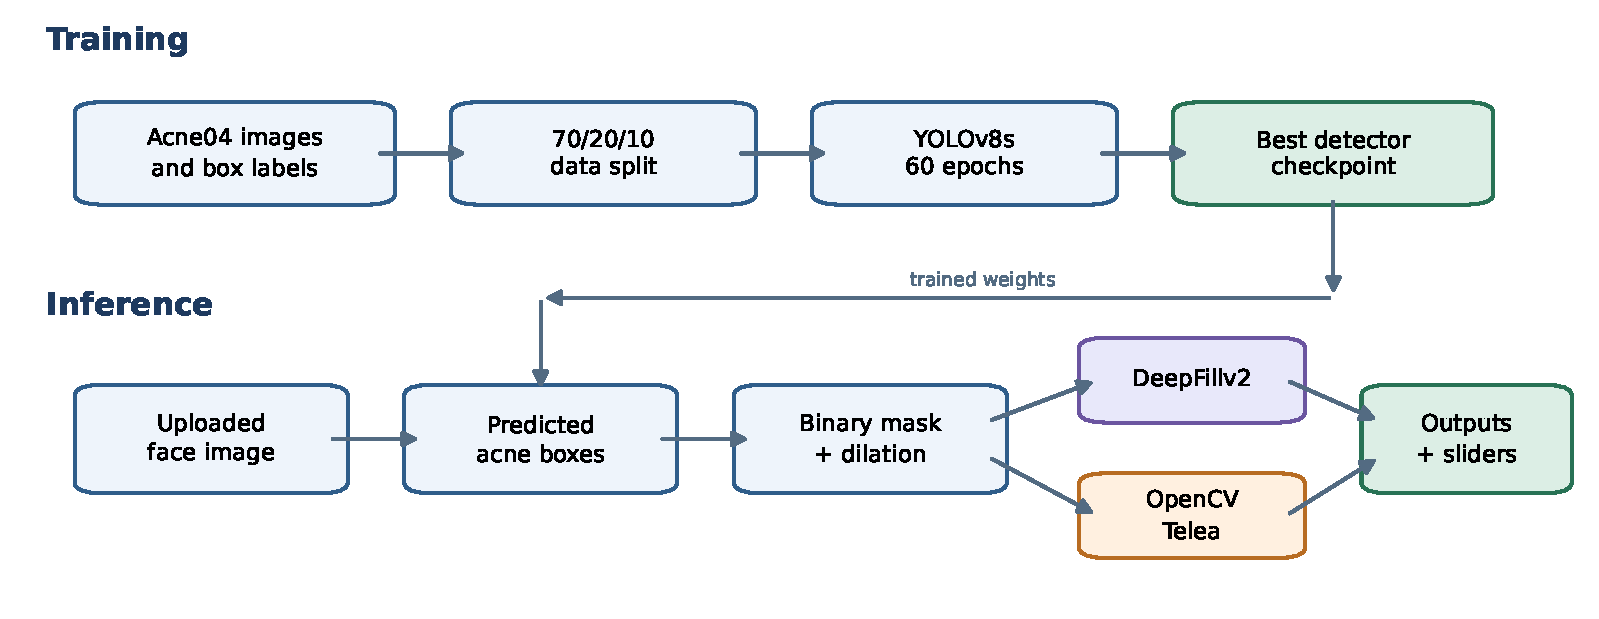
\includegraphics[width=\textwidth]{figures/method_overview.pdf}
    \caption{Overview of the proposed system. Acne04 box annotations train
    YOLOv8s. At inference time, the checkpoint localizes acne in an uploaded
    face, a dilated mask selects the edit regions, and DeepFillv2 and OpenCV
    Telea restore the same masked input.}
    \label{fig:overview}
\end{figure*}

\subsection{Dataset preparation and detector training}

The Acne04 YOLOv8-format dataset \cite{acne04} contains 1,457 image/label
pairs used in this run. Each label file stores pimple boxes in YOLO format.
The training script sorts the paired files and applies two
\texttt{train\_test\_split} calls with random state 42. This produces
1,019 training, 292 validation, and 146 test images, approximately a
70/20/10 split. The test images are withheld from parameter updates and
checkpoint selection.

The detector starts from Ultralytics' pretrained \texttt{yolov8s.pt}
weights and is trained for 60 epochs at 640-pixel input size, batch size
16, and AdamW optimization. The implemented augmentations include
rotation up to 10 degrees, translation 0.1, scale 0.5, horizontal flip
probability 0.5, mosaic 1.0, mixup 0.1, random erasing 0.4, and
hue/saturation/value adjustments of 0.015/0.7/0.4. Vertical flip is
disabled because an upside-down face is unlikely in the intended use.
The run saves the best checkpoint as
\texttt{models/acne04\_60\_best.pt}; the app loads it by default.

\subsection{Detection and mask construction}
\label{sec:mask}

For an input image $I$ with height $H$ and width $W$, YOLOv8s predicts a
set of boxes $B_{\tau}=\{b_i\}$ after a confidence threshold $\tau$.
Each accepted box is filled into an initially zero-valued image. The
source-resolution mask is
\begin{equation}
M_0(x,y)=
\begin{cases}
1,& (x,y)\in \bigcup_{b_i\in B_{\tau}} b_i,\\
0,& \text{otherwise}.
\end{cases}
\end{equation}
The app then applies a square morphological dilation kernel $K$ for $r$
iterations, giving $M=\operatorname{dilate}_{K}^{r}(M_0)$. Dilation allows
the fill to cover lesion edges just outside the predicted rectangle.
The default controls are $\tau=0.10$, a $9\times9$ kernel, and $r=3$.
These parameters are adjustable in the interface. A box is a coarse
localization, so dilation can also include unaffected skin; the threshold
and mask size therefore have a visible effect on the outcome.

\subsection{Two inpainting paths}

Both methods use the same input image and mask resized to
$512\times512$ pixels. DeepFillv2 uses a pretrained gated-convolution
generator \cite{yu2019}. The application downloads its inference code and
weights on first launch, writes the image and mask to the expected input
paths, runs the upstream inference script, and reads its output. This
project did not retrain DeepFillv2.

The comparison path calls
\texttt{cv2.inpaint(image, mask, 3, cv2.INPAINT\_TELEA)}, where 3 is the
inpainting radius in pixels. Telea inpainting propagates nearby image
information into masked regions \cite{telea2004}; it has no learned
weights or training epochs. Keeping $I$ and $M$ fixed makes the two
outputs directly comparable for this input, although the methods may
behave differently on large or irregular masks.

\subsection{User interaction}

The Gradio app accepts an RGB face image and exposes controls for
confidence, dilation kernel size, and dilation iterations. It shows the
DeepFillv2 and OpenCV outputs separately. One draggable slider compares
the original with DeepFillv2; a second compares OpenCV with DeepFillv2.
If no acne boxes pass the confidence threshold, the app returns the
original image rather than forcing an inpainting result.

\section{Experimental Protocol}
\label{sec:experiments}

The experiments comprise a 60-epoch detector training run, validation
metrics recorded at each epoch, a separate evaluation of the saved best
checkpoint on the test split, and qualitative inpainting comparisons.
Table~\ref{tab:setup} records the principal settings. The complete
per-epoch CSV and best checkpoint are available in the project
repository \cite{projectrepo}.

\begin{table}[t]
    \centering
    \small
    \begin{tabular}{p{0.38\columnwidth}p{0.50\columnwidth}}
        \toprule
        Setting & Value\\
        \midrule
        Dataset & Acne04 YOLOv8, 1,457 pairs\\
        Train / validation / test & 1,019 / 292 / 146 images\\
        Detector & YOLOv8s, pretrained initialization\\
        Training & 60 epochs, AdamW, batch 16\\
        Detector input & 640 pixels\\
        Inpainting output & $512\times512$ pixels\\
        Default mask & $\tau=0.10$, $9\times9$, 3 dilations\\
        OpenCV radius & 3 pixels, Telea method\\
        \bottomrule
    \end{tabular}
    \caption{Dataset and implementation settings.}
    \label{tab:setup}
\end{table}

Precision and recall evaluate predicted acne boxes. Average precision
integrates the precision--recall relation at a chosen
intersection-over-union (IoU) match threshold. We report mAP@50 at
IoU $0.50$ and mAP@50:95 averaged over IoU thresholds $0.50$ through
$0.95$. The training file does not provide a separate mAP@95 value.
These metrics quantify detection, not visual restoration quality.

\section{Results and Analysis}
\label{sec:results}

\subsection{Validation over 60 epochs}

Figure~\ref{fig:curves} plots all 60 recorded validation points.
Table~\ref{tab:epochs} gives representative epochs. Validation mAP@50
rose from 0.01\% at epoch 1 to 32.53\% at epoch 57, with dips and
recoveries rather than a monotonic increase. Epoch 57 also had the
highest recorded mAP@50:95, 8.00\%. At epoch 60, precision was
slightly higher (40.43\%), while recall, mAP@50, and mAP@50:95 were
slightly lower than at epoch 57. This supports using the saved best
checkpoint rather than assuming the final epoch is best. The gap
between mAP@50 and mAP@50:95 suggests that accurate, tight localization
remains difficult for small lesions.

\begin{figure*}[t]
    \centering
    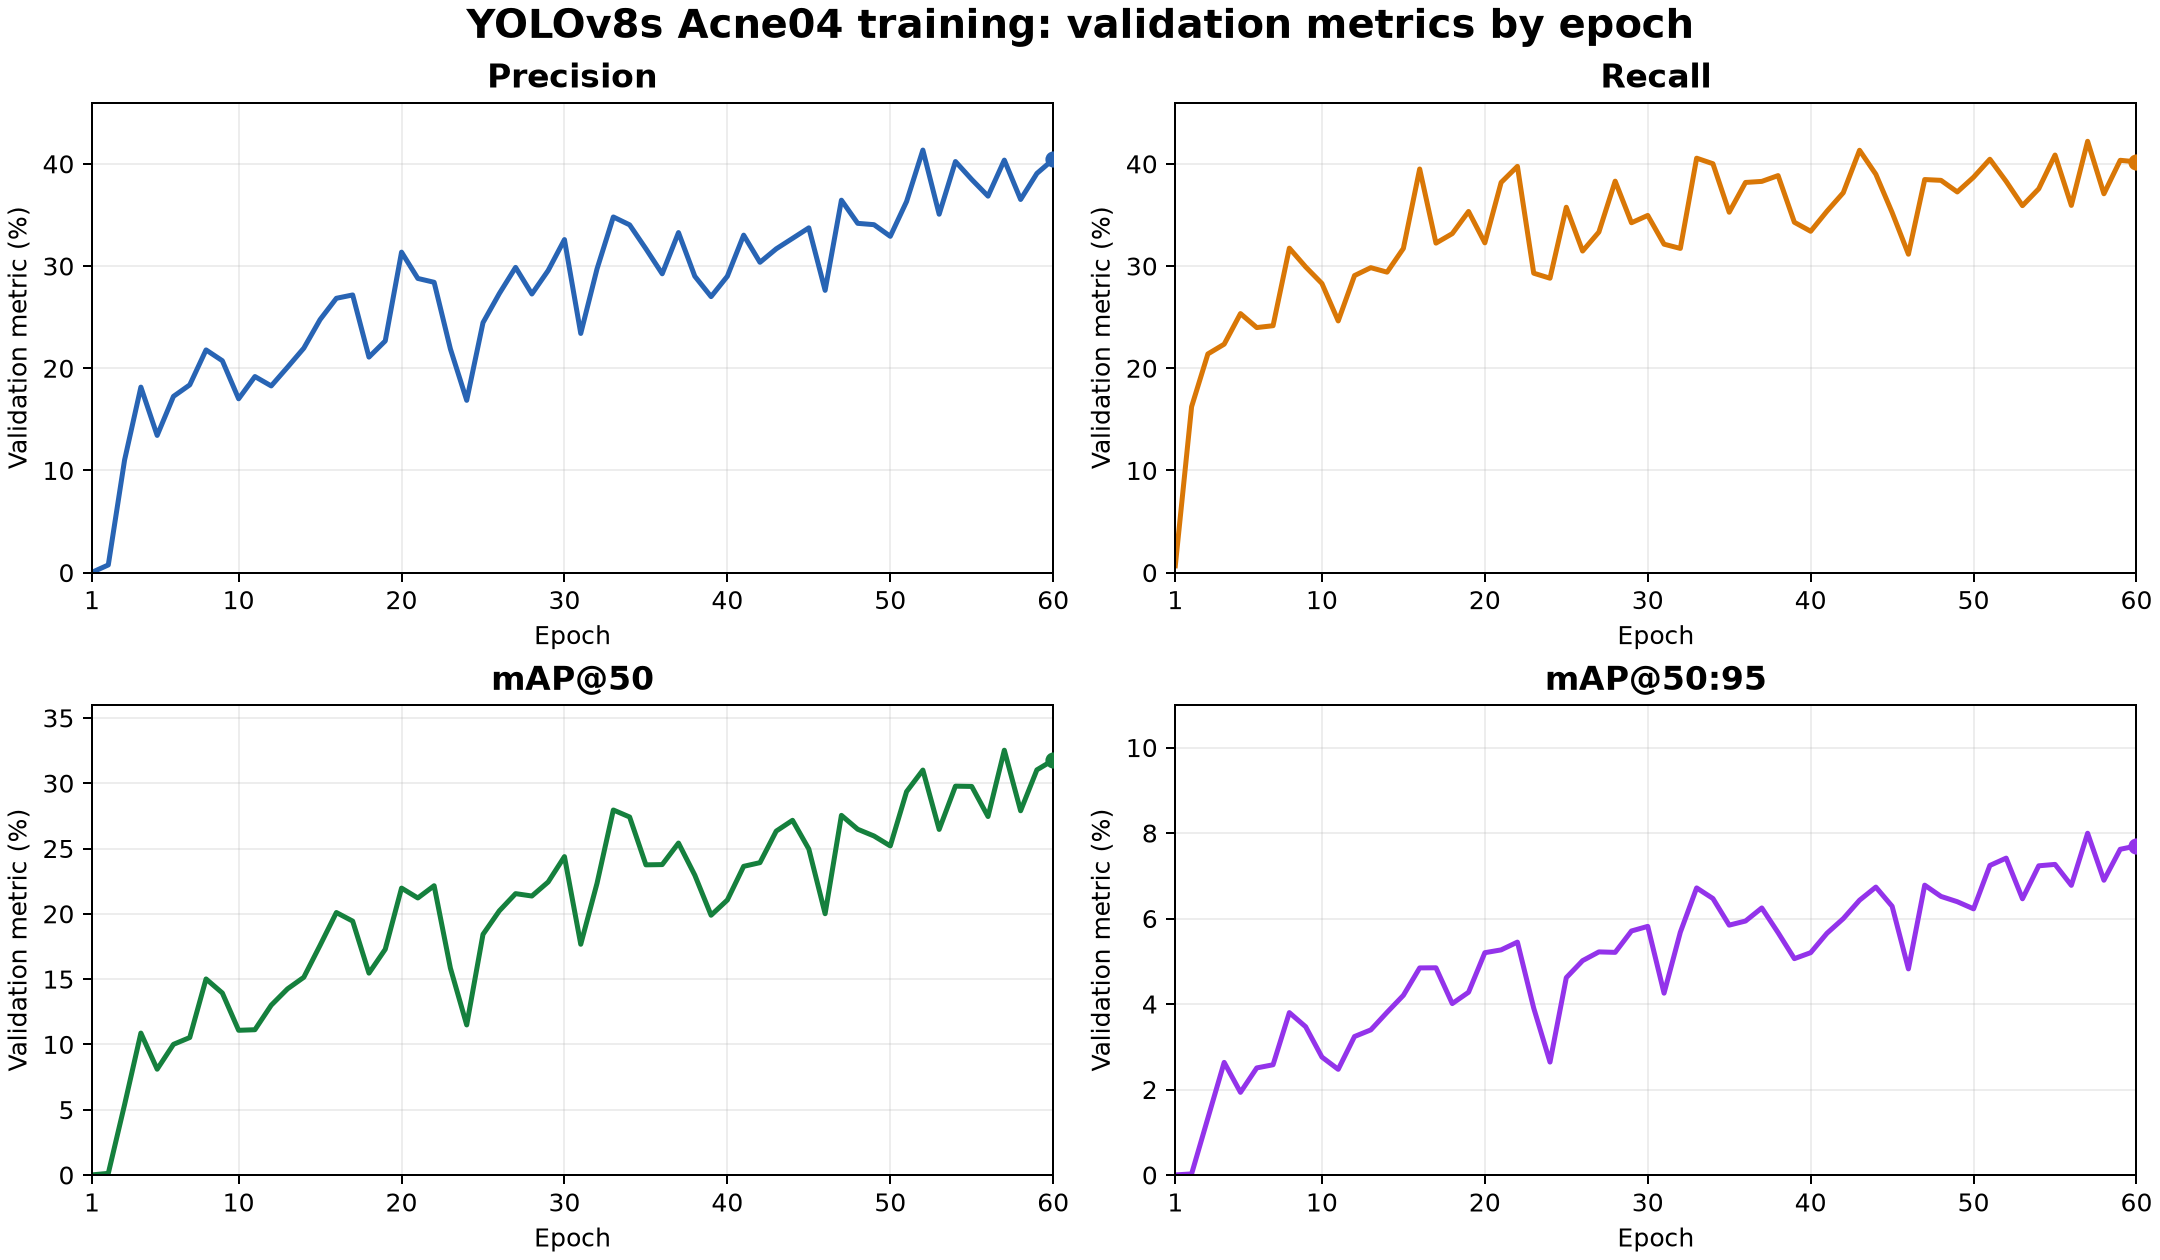
\includegraphics[width=0.92\textwidth]{figures/training_metrics.png}
    \caption{Validation precision, recall, mAP@50, and mAP@50:95 for
    each of the 60 YOLOv8s training epochs. Values are taken directly
    from the recorded \texttt{results.csv}.}
    \label{fig:curves}
\end{figure*}

\begin{table}[t]
    \centering
    \small
    \setlength{\tabcolsep}{4pt}
    \begin{tabular}{rcccc}
        \toprule
        Epoch & P & R & mAP$_{50}$ & mAP$_{50:95}$\\
        \midrule
        1 & 0.03 & 0.67 & 0.01 & 0.00\\
        10 & 17.01 & 28.29 & 11.08 & 2.76\\
        20 & 31.36 & 32.27 & 21.97 & 5.20\\
        30 & 32.59 & 34.95 & 24.38 & 5.82\\
        40 & 29.00 & 33.40 & 21.06 & 5.20\\
        50 & 32.91 & 38.69 & 25.20 & 6.23\\
        \textbf{57} & \textbf{40.37} & \textbf{42.20}
          & \textbf{32.53} & \textbf{8.00}\\
        60 & 40.43 & 40.19 & 31.77 & 7.70\\
        \bottomrule
    \end{tabular}
    \caption{Validation detection metrics in percent. P is precision
    and R is recall; epoch 57 is the saved best checkpoint.}
    \label{tab:epochs}
\end{table}

\subsection{Held-out detector evaluation}

The saved checkpoint was evaluated once on the 146-image test split,
which contains 1,776 labeled lesion instances.
Table~\ref{tab:test} compares this held-out result with the recorded
epoch-57 validation result. Test mAP@50 is 32.79\%, close to
the validation value of 32.53\%; the other test metrics are also
slightly higher. This is evidence for the detector on this particular
held-out split, not a guarantee for different lighting, cameras, skin
tones, or acne types. No repeated random splits or confidence intervals
were computed.

\begin{table}[t]
    \centering
    \small
    \setlength{\tabcolsep}{4pt}
    \begin{tabular}{lcccc}
        \toprule
        Split & P & R & mAP$_{50}$ & mAP$_{50:95}$\\
        \midrule
        Validation, epoch 57 & 40.37 & 42.20 & 32.53 & 8.00\\
        Test, best checkpoint & 42.39 & 42.74 & 32.79 & 8.51\\
        \bottomrule
    \end{tabular}
    \caption{Detection metrics in percent on the validation and
    held-out test splits. The test row is from a separate evaluation
    of \texttt{models/acne04\_60\_best.pt}.}
    \label{tab:test}
\end{table}

\subsection{Mask and restoration comparison}

Figure~\ref{fig:outcome} shows an actual result for
\texttt{levle1\_203.jpg}, an image in the test split. At the default
confidence and dilation settings, the detector produced 26 boxes and
the resulting source-resolution mask covered 3.93\% of the image.
The white mask regions are exactly the areas targeted for filling.
DeepFillv2 reduced several visible lesions while keeping more
continuous nearby skin in this example. The OpenCV result removed
content inside the same mask but shows conspicuous smooth patches
around some rectangles. The observation is qualitative and applies
to the displayed example; it is not a measured superiority claim
across the dataset.

\begin{figure*}[t]
    \centering
    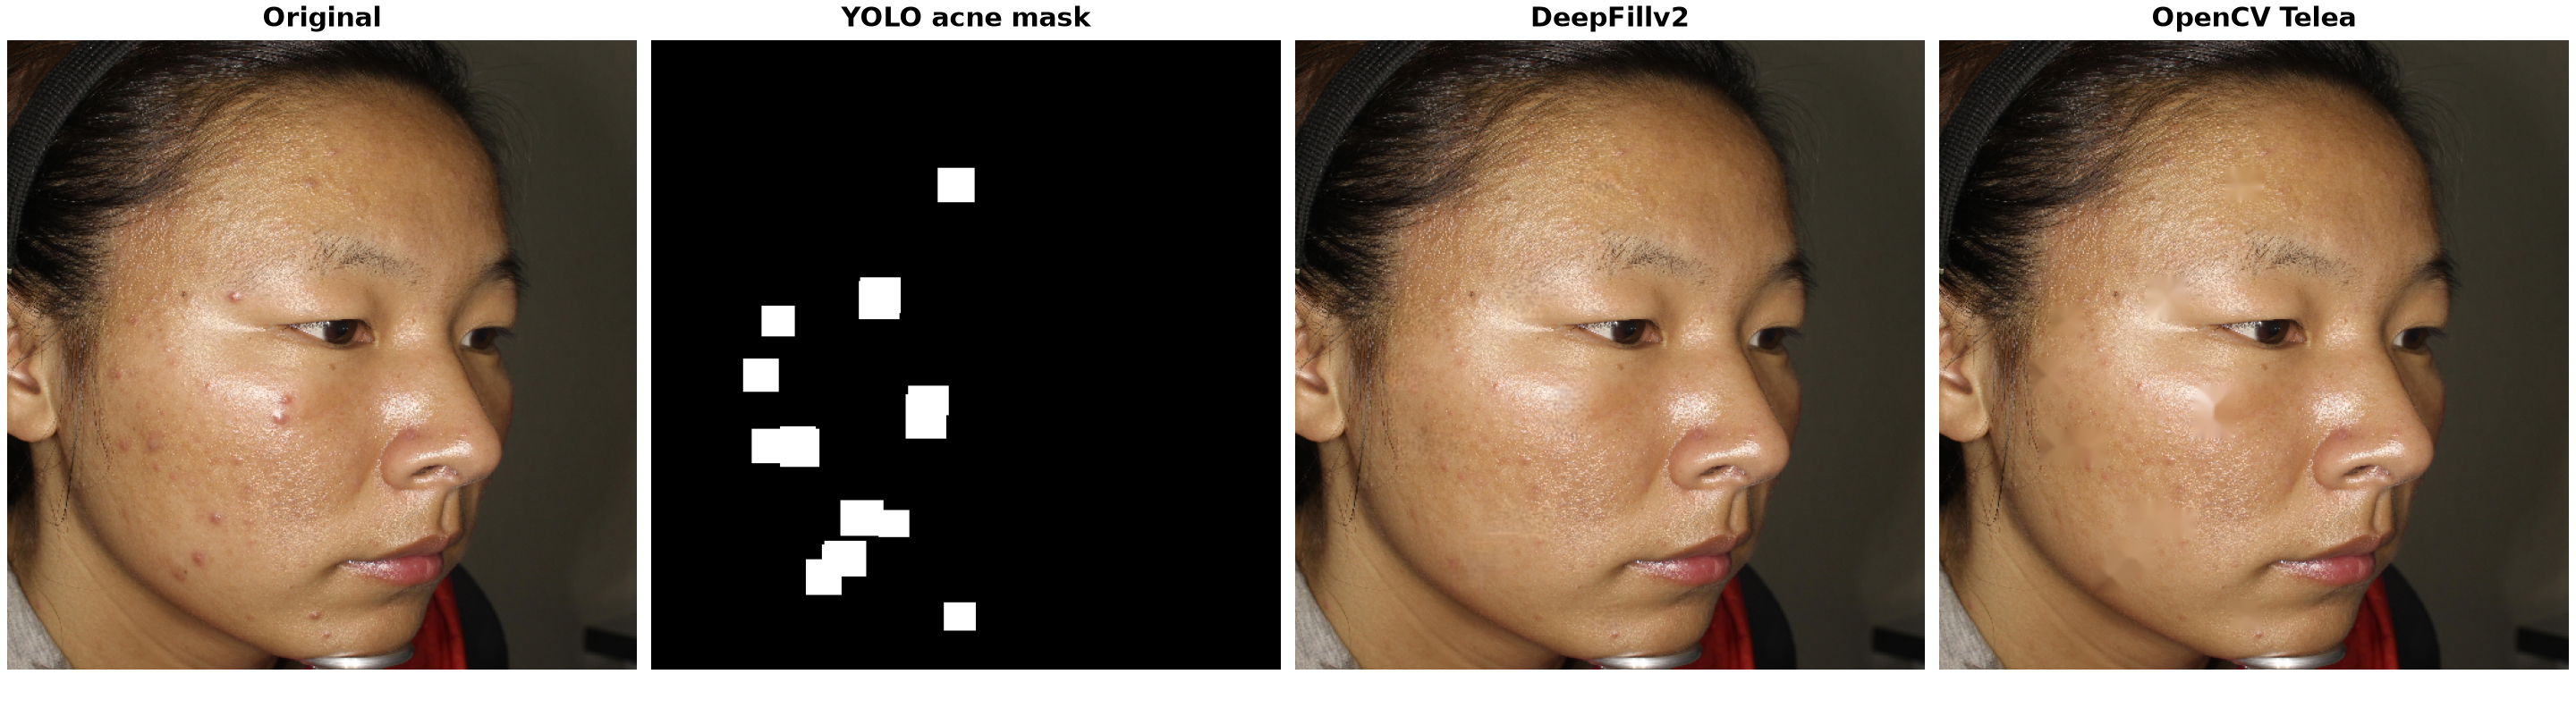
\includegraphics[width=\textwidth]{figures/project_outcome.png}
    \caption{Held-out Acne04 test image, predicted and dilated acne
    mask, DeepFillv2 result, and OpenCV Telea result. Settings:
    confidence 0.10, $9\times9$ dilation kernel, three dilation
    iterations, and Telea radius 3 pixels.}
    \label{fig:outcome}
\end{figure*}

As a small mask-sensitivity diagnostic, the test image
\texttt{levle1\_0.jpg} was processed with two confidence thresholds
while keeping the $9\times9$ kernel and three dilation iterations
fixed. Table~\ref{tab:mask} shows that lowering the threshold from
0.10 to 0.05 increased the accepted boxes from 62 to 158 and the
masked area from 18.82\% to 27.39\%. This illustrates why the
interface exposes the threshold: an overly permissive detector can
remove much more skin than intended. The diagnostic uses one image,
so it does not estimate average threshold sensitivity.

\begin{table}[t]
    \centering
    \small
    \begin{tabular}{ccc}
        \toprule
        Confidence & Accepted boxes & Masked area (\%)\\
        \midrule
        0.05 & 158 & 27.39\\
        0.10 & 62 & 18.82\\
        \bottomrule
    \end{tabular}
    \caption{Mask sensitivity on one held-out image,
    \texttt{levle1\_0.jpg}. Other mask settings were fixed.}
    \label{tab:mask}
\end{table}

\section{Limitations and Conclusion}
\label{sec:conclusion}

The detector uses boxes, not pixel-level lesion segmentation. Boxes
and their dilation may mask normal skin, and missed detections leave
lesions untouched. Resizing every input to $512\times512$ for
inpainting can distort non-square portraits. The example in
Figure~\ref{fig:outcome} exposes a limitation of the classical
baseline on these rectangular masks, but the dataset has no paired
clean target images. Consequently, PSNR, SSIM, or a defensible
dataset-wide ranking of inpainting quality cannot be reported from
these data. Neither the DeepFillv2 generator nor OpenCV Telea was
trained on Acne04 in this project; the 60-epoch result applies to
YOLOv8s only. The tool is for visual editing, not medical diagnosis.

This project delivers a working and inspectable acne-removal pipeline:
an Acne04-trained detector creates a mask, two established
inpainting methods fill the same regions, and sliders let users
inspect their results. The held-out detector mAP@50 is 32.79\%.
Future work should use pixel-level masks, assess performance across
more varied portraits, and collect paired or human-rated restoration
targets before making stronger claims about the comparative visual
quality of the two methods.

\section{Datasets and Source Repositories}
\label{sec:links}

The following links identify every dataset and source repository
used directly in this project or its report:
\begin{itemize}
    \item Project code and trained checkpoint:
    \href{https://github.com/blackleg-sanji007/pimple-removal-tool/tree/main}{Pimple Removal Tool on GitHub}
    \cite{projectrepo}.
    \item Training images and YOLO box labels:
    \href{https://www.kaggle.com/datasets/shreyash1110/acne04-yolov8}{Acne04 YOLOv8 on Kaggle}
    \cite{acne04}.
    \item Pipeline reference:
    \href{https://github.com/architk22/EE604-Course-Project}{EE604 Course Project}
    \cite{architrepo}.
    \item Pretrained inpainting implementation and weights:
    \href{https://github.com/vrindaprabhu/deepfillv2_colab}{deepfillv2\_colab}
    \cite{deepfillrepo}.
    \item Detector framework:
    \href{https://github.com/ultralytics/ultralytics}{Ultralytics repository}
    \cite{ultralytics}.
    \item Classical inpainting library:
    \href{https://github.com/opencv/opencv}{OpenCV repository}
    \cite{opencvdocs}.
    \item Other project dependencies:
    \href{https://github.com/gradio-app/gradio}{Gradio},
    \href{https://github.com/pytorch/pytorch}{PyTorch},
    \href{https://github.com/numpy/numpy}{NumPy},
    \href{https://github.com/scikit-learn/scikit-learn}{scikit-learn},
    \href{https://github.com/wkentaro/gdown}{gdown},
    \href{https://github.com/tqdm/tqdm}{tqdm}, and
    \href{https://github.com/scikit-image/scikit-image}{scikit-image}.
    \item Report figures:
    \href{https://github.com/matplotlib/matplotlib}{Matplotlib}.
    \item Report format:
    \href{https://github.com/cvpr-org/author-kit}{CVPR author kit}
    \cite{cvprkit}.
\end{itemize}

{\small
\bibliographystyle{ieeenat_fullname}
\bibliography{main}
}

\clearpage
\appendix
\onecolumn
\section{Complete Project-Authored Code}
\label{app:code}

The following listings include the complete Python application and
training script in the project repository, plus their dependency
file. The binary detector checkpoint is available through the
\href{https://github.com/blackleg-sanji007/pimple-removal-tool/tree/main/models}{project repository}.
The externally maintained DeepFillv2 implementation is downloaded
by the app and is linked in Section~\ref{sec:links}; it is not
project-authored code. The listings are frozen copies for this report.

\subsection{Application: \texttt{app.py}}
\lstinputlisting[language=Python]{code/app.py}

\subsection{Detector training: \texttt{train\_acne04.py}}
\lstinputlisting[language=Python]{code/train_acne04.py}

\subsection{Dependencies: \texttt{requirements.txt}}
\lstinputlisting{code/requirements.txt}

\end{document}
